\subsection{Baza PostgreSQL}
\subsubsection{Diagram encji}
\begin{figure}[h]
 \centering
 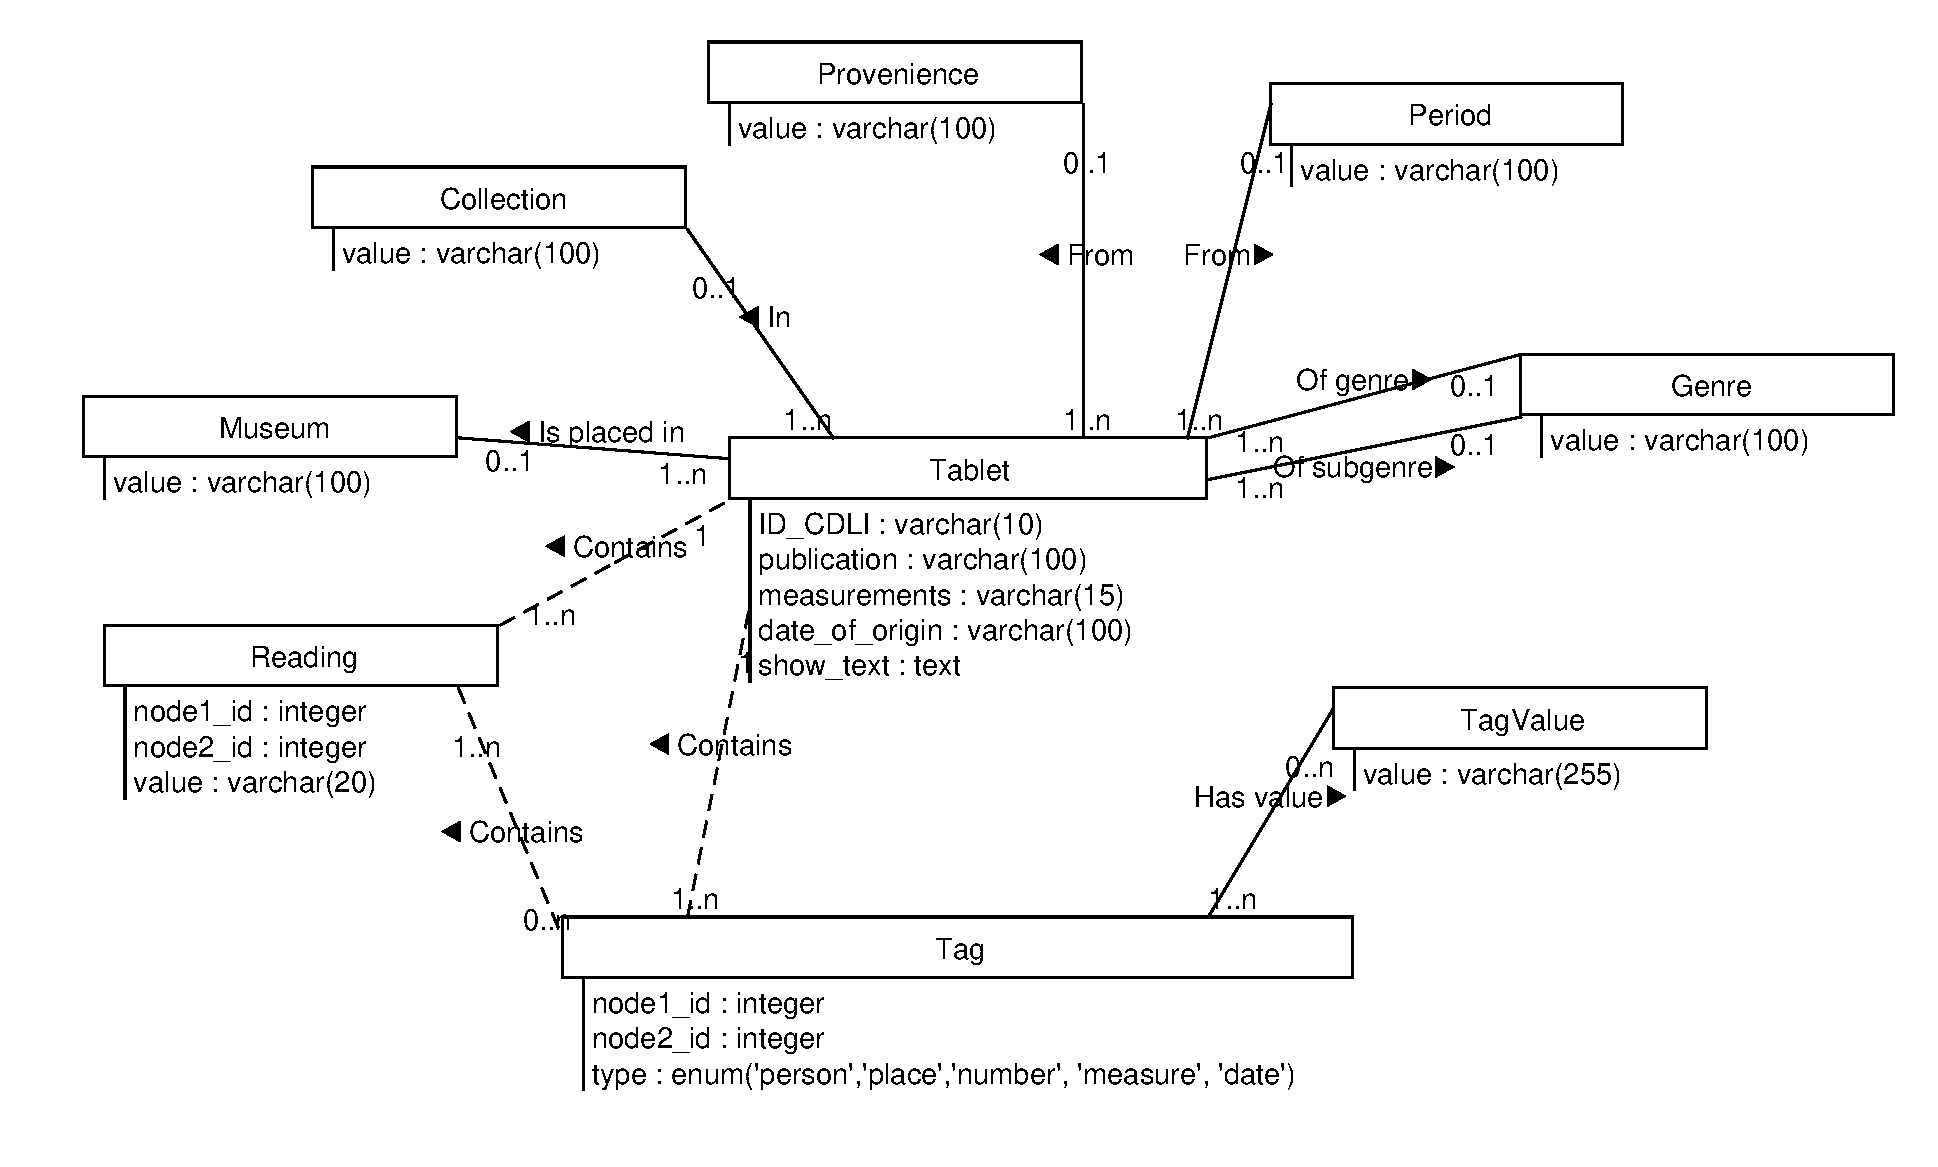
\includegraphics[width=500px,bb=0 0 930 560]{../diagramy/diagram-encji-maly.pdf}
 % diagram-encji-maly.pdf: 930x560 pixel, 72dpi, 32.81x19.76 cm, bb=0 0 930 560
 \caption{Diagram encji}
\end{figure}
Jednym z problemów przy projektowaniu bazy danych był wybór takiej reprezentacji treści tabliczki, żeby efektywnie wykonywać następujące operacje:
\begin{itemize}
 \item wyszukiwanie po treści tabliczki (po odczytach, klinach i tagach),
\item wyszukiwanie treści konkretnej tabliczki.
\end{itemize}
Najlepszym rozwiązaniem pierwszego problemu jest reprezentacja treści tabliczki
w formie grafu,
 którego krawędziami są odczyty, kliny i tagi (zgodnie z pomysłem dr Wojciecha Jaworskiego\cite[s.13-24]{jaworski}).
Natomiast w przypadku drugiego problemu narzuca się przechowywanie treści
jako otwarty tekst.
Zdecydowałyśmy się na połączenie obu sposobów. Odczyty, kliny i tagi przechowujemy w tabelach Reading, Cuneiform i Tag, 
natomiast otwarty tekst w kolumnie show\_text tabeli Tablet.
Aby zapewnić możliwość odwzorowania treści tabliczki między reprezentacjami, węzły są liczbami postaci:
%Treść tabliczki jest przechowywana nie tylko jako otwarty tekst (kolumna w tabeli Tablet), ale także w formie grafu,
 %którego krawędziami są odczyty i tagi (zgodnie z pomysłem dr Wojciecha Jaworskiego\cite[s.13-24]{jaworski}) 
%w tabelach Reading i Tag. 
%  Węzeł tego grafu jest liczbą postaci:
\begin{verbatim}
 <numer węzła w tabliczce> * 1 000 000 + <id tabliczki>
\end{verbatim}
gdzie numer węzła w tabliczce to numer kolejnego słowa (słowa są oddzielone spacjami i końcem linii) pomnożone przez 10 (żeby umożliwić
wstawienie kilku węzłów w jednym słowie np. pozwolić na przetłumaczenie jednego słowa na sekwencję trzech klinów). 


Przerywane linie na diagramie encji oznaczają opisany powyżej związek pomiędzy id węzła (node1\_id i node2\_id) 
a id tabliczki (Tablet.id).

% relacja
% Stąd wzięły się przerywane linie na diagramie encji - nie ma bezpośredniego klucza obcego w tabeli Reading (czy Tag) do Tablet, 
% jednak związek istnieje. Taki sposób przechowywania informacji o treści tabliczki umożliwia sprawniejsze wyszukiwanie nie tylko
% po odczytach (pozwala pomijać linie z uszkodzeniami) ale także w przyszłości ułatwia zaimplementowanie wyszukiwania po klinach,
% po tagach itp.
% Poza sprawnym
%  wyszukiwaniem ułatwia to rozszerzenie programu o możliwość wyszukiwania po klinach - po dodaniu tabeli Cuneiform.

 

\subsubsection{Translator\_config}
Tłumaczy otrzymane fragmenty drzewa struktury zapytania na język SQL. Przetłumaczone fragmenty zbiera do buforów 
(\textit{select}, \textit{from}, \textit{where}), które następnie odpowiednio łączy.
Każde proste zapytanie TQL jest tłumaczone na pojedyncze zapytanie SQL. Tłumaczenie kilku prostych zapytań
łączone jest za pomocą UNION.

\subsubsection{Inicjalizacja zapytania}
Tłumaczenie prostego zapytania zaczyna się od inicjalizacji buforów przechowujących poszczególne części wynikowego SQL-a.
\textit{select} jest inicjowany na 
\begin{verbatim}
SELECT t.id, t.id_cdli, t.publication, t.measurements, t.origin_date, 
       p.value as provenience, pd.value as period,
       g1.value as genre, g2.value as subgenre, 
       c.value as collection, t.text
\end{verbatim}
\textit{from} jest inicjowany
\begin{verbatim}
FROM tablet t
  LEFT JOIN provenience p ON p.id=t.provenience_id
  LEFT JOIN collection c ON c.id=t.collection_id
  LEFT JOIN genre g1 ON g1.id=t.genre_id
  LEFT JOIN genre g2 ON g2.id = t.subgenre_id
  LEFT JOIN period pd ON pd.id = t.period_id
\end{verbatim}
\textit{where} początkowo zawiera pusty ciąg znaków.



\subsubsection{Tłumaczenie konstrukcji prostych}
Poniższe tłumaczenia są dodawane do bufora \textit{where} i łączone za pomocą AND.
\begin{longtable}{|p{3in}|p{3in}|}
\hline
{\bf Konstrukcja} & {\bf Tłumaczenie na SQL}\\
\hline
\endhead
provenience: wartosc & \begin{verbatim}p.value LIKE 'wartosc'\end{verbatim}
\\
\hline
publication: wartosc & 
\begin{verbatim}
t.publication LIKE 'wartosc'
\end{verbatim}
\\
\hline
period: wartosc & 
\begin{verbatim}
pd.value LIKE 'wartosc'
\end{verbatim}
\\
\hline
year: wartosc & 
\begin{verbatim}
t.origin_date LIKE 'wartosc'
\end{verbatim}
\\
\hline
genre: wartosc & 
\begin{verbatim}
   g1.value LIKE 'wartosc' 
OR g2.value LIKE 'wartosc'
\end{verbatim}
\\
\hline
cdli\_id: wartosc & 
\begin{verbatim}
t.cdli_id LIKE 'wartosc'
\end{verbatim}
\\
\hline
museum: wartosc & 
\begin{verbatim}
t.museum LIKE 'wartosc'
\end{verbatim}
\\
\hline
collection: wartosc & 
\begin{verbatim}
c.value LIKE 'wartosc'
\end{verbatim}
\\
\hline
\end{longtable}

\textbf{Tłumaczenie operatorów:}
\begin{longtable}{|p{1in}|p{1in}|}
\hline
{\bf Operator} & {\bf Tłumaczenie}\\
\hline
\endhead
/ & OR\\ 
\hline
-- & NOT\\ 
\hline
+ & AND\\ 
\hline
* & \%  \\ 
\hline
\end{longtable}


\subsubsection{Tłumaczenie konstrukcji złożonych}
%Została zaimplementowana tylko jedna konstrukcja złożona - przy zapytaniu o treść tabliczki (pole ''text``).
Przy tłumaczeniu konstrukcji złożonych
korzystamy z przedstawienia treści tabliczki w formie grafu.

Pojawienie się wyszukiwania po treści tabliczki niesie za sobą konieczność dodania do bufora \textit{from}:
\begin{verbatim}
INNER JOIN (
  <wynikowe zapytanie o treść tablczki>
) AS sequence ON sequence.id_tab = t.id
\end{verbatim}

natomiast do \textit{select} dodajemy:
\begin{verbatim}
, sequence.nodes as nodes
\end{verbatim}

gdzie $<$wynikowe zapytanie o treść tablczki$>$ to kombinacja zapytań typu:
\begin{verbatim}
  SELECT 
    id_tab, 
    CAST(array_accum(nodes) as TEXT) as nodes, 
    COUNT(DISTINCT id_seq) AS seq, 
    <id_seq> AS id_seq
  FROM (
    SELECT
      t1.node1_id % 1000000 AS id_tab,
      '{' || t1.node1_id || ',' || t<dl_sekw>.node2_id || '}' AS nodes,
      1 AS id_seq
    FROM
      <nazwa_tabeli> t1
      LEFT JOIN <nazwa_tabeli> t2 ON (t2.node1 = t1.node2)
      LEFT JOIN <nazwa_tabeli> t3 ON (t3.node1 = t2.node2)
      ...
      LEFT JOIN <nazwa_tabeli> t<dl_sekw> ON (t<dl_sekw>.node1 = t<dl_sekw-1>.node2)
   WHERE
      t1.value LIKE '<sekw[1]>'
     AND
      t2.value LIKE '<sekw[2]>'
    AND
      t3.value LIKE '<sekw[3]>'
    AND
      ...
    AND
      t<dl_sekw>.value LIKE '<sekw[<dl_sekw>]>'
   ) AS a 
  GROUP BY id_tab
\end{verbatim}
Zmienne użyte w powyższym pseudo-kodzie:
\begin{description}
 \item[id\_sekw] - kolejny numer sekwencji (przydatny przy bardziej skomplikowanym zapytaniu - do rozróżniania podzapytań)
 \item[dl\_sekw] - ilość słów składających się na wyszukiwaną sekwencję
 \item[sekw] - tablica zawierająca słowa składające się na wyszukiwaną sekwencję
\item[nazwa\_tabeli] - nazwa tabeli, w której wyszukujemy (Reading lub Cuneiform)
 \end{description}

\begin{longtable}{|p{1in}|p{4.5in}|}
\hline
{\bf Operator} & {\bf Tłumaczenie}\\
\hline
\endhead
/ & 
\begin{verbatim}
SELECT 
  id_tab, 
  CAST(array_accum(nodes) as TEXT) as nodes, 
  COUNT(DISTINCT id_seq) as seq,
  <id_sekw> as id_seq
FROM 
(
  <zapytanie1>
  UNION
  <zapytanie2>
)
as c
GROUP BY id_tab
\end{verbatim}
\\ 
\hline
+ &
\begin{verbatim}
SELECT * FROM
 (SELECT id_tab, 
         CAST(array_accum(nodes) as TEXT) as nodes, 
         COUNT(DISTINCT id_seq) as seq, 
         <id_sekw> as id_seq
  FROM
    (<zapytanie1>
    UNION
    <zapytanie2>)
  as c 
  GROUP BY id_tab
 ) as b
WHERE b.seq=2 
\end{verbatim}
\\ 
\hline
-- & 
\begin{verbatim}
SELECT 
  id_tab, 
  '' as wezly, 
  0 as sekw,
  <id_sekw> as id_sekw
FROM
(
 (SELECT id as id_tab from tabliczka)
 EXCEPT
 (SELECT id_tab from
    <zapytanie_negowane> as a
 )   
) as b
\end{verbatim}
\\ 
\hline
* & \%  \\ 
\hline
\end{longtable}


\subsubsection{Database\_config}

Odpowiada za wywołanie zapytania na konkretnej bazie i zapisanie wyniku do struktury Tablets.
 Korzysta z pliku database.conf, który zawiera dane dostępu do bazy (host, port, użytkownik, hasło, nazwa bazy)
oraz biblioteki libpq-fe.h do PostgreSQL.
